\subsection{Nono sprint}

\begin{minipage}{\textwidth}
  Di seguito è riportata la distribuzione delle ore per ciascun membro del team, accumulate in totali per persona e per ruolo:
  \begin{table}[H]
    \begin{tabularx}{\textwidth}{|c|*{6}{>{\centering}X|}c|}
      \hline
      \multicolumn{8}{|c|}{\textbf{Consuntivo orario}} \\
      \hline
      \textbf{Membro del team} & \textbf{Re} & \textbf{Am} & \textbf{An} & \textbf{Pt} & \textbf{Pr} & \textbf{Ve} & \textbf{Totale per persona} \\
      \hline
      Cavalli Riccardo & 0 & 0 & 0 & 2 & 1 & 2 & 5 \\
      \hline
      Pianon Raul & 0 & 2 & 0 & 1 & 0 & 1 & 4 \\
      \hline
      Dall’Amico Martina & 1 & 0 & 0 & 0 & 0 & 3 & 4 \\
      \hline
      Cristo Marco & 0 & 2 & 0 & 0 & 0 & 2 & 4 \\
      \hline
      Lewental Sebastiano & 2 & 0 & 0 & 0 & 0 & 2 & 4 \\
      \hline
      Zecchinato Mattia & 0 & 0 & 0 & 2 & 0 & 2 & 4 \\
      \hline
      Stocco Tommaso & 0 & 0 & 0 & 0 & 1 & 3 & 4 \\
      \hline
      \textbf{Totale ore per ruolo} & 3 & 4 & 0 & 6 & 1 & 15 & \textbf{29} \\
      \hline
    \end{tabularx}
    \caption{Sprint 10 - Consuntivo orario}
  \end{table}
  \end{minipage}

  \begin{figure}[H]
    \centering
    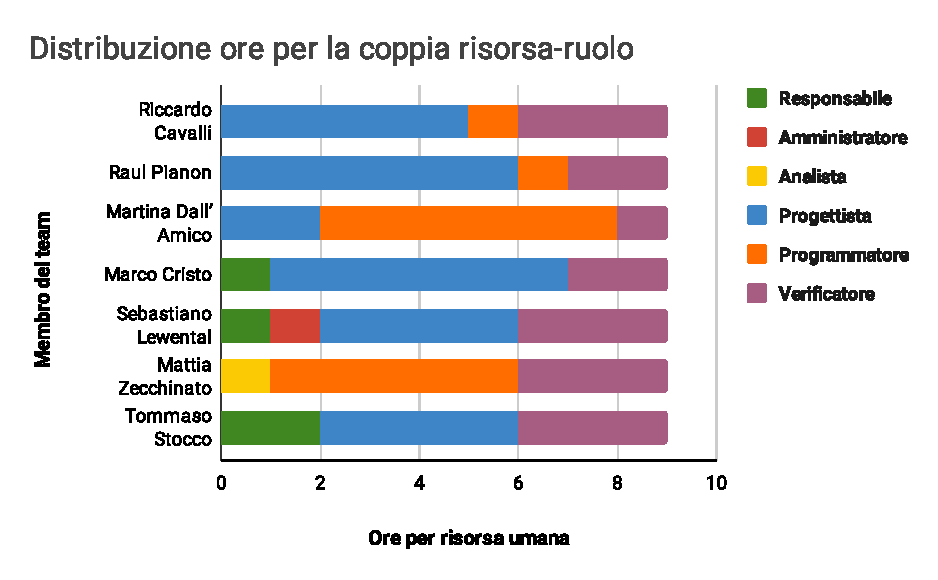
\includegraphics[width=0.90\textwidth]{assets/Consuntivo/Sprint-10/distribuzione_ore_risorsa_ruolo.pdf}
    \caption{Sprint 10 - Istogramma della distribuzione oraria per la coppia risorsa-ruolo}
  \end{figure}

  \begin{figure}[H]
    \centering
    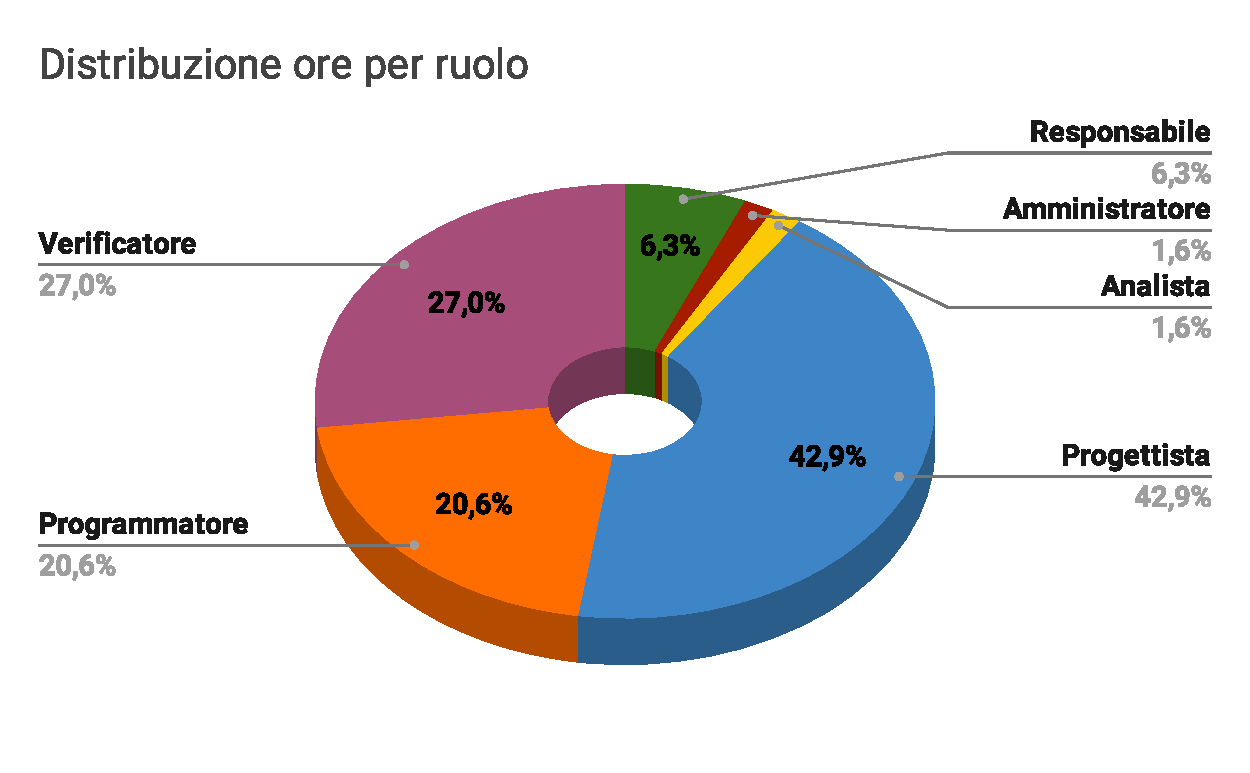
\includegraphics[width=0.90\textwidth]{assets/Consuntivo/Sprint-10/distribuzione_ore_ruolo.pdf}
    \caption{Sprint 10 - Areogramma della distribuzione oraria per ruolo}
  \end{figure}

  \begin{minipage}{\textwidth}
  Di seguito è riportato il consuntivo economico del nono \glossario{sprint}:
  \begin{table}[H]
  \begin{adjustwidth}{-0.5cm}{-0.5cm}
    \centering
    \begin{tabular}{|P{2.9cm}|P{2.3cm}|P{2.5cm}|P{2.3cm}|>{\arraybackslash}P{2.5cm}|}
      \hline
      \multicolumn{5}{|c|}{\textbf{Consuntivo economico}} \\
      \hline
      \textbf{Ruolo} & \textbf{Ore per ruolo} & \textbf{Delta ore preventivo - consuntivo} & \textbf{Costo (in \texteuro)} & \textbf{Delta costo preventivo - consuntivo (in \texteuro)} \\
      \hline
      \Responsabile[U]{} & 3 & 0 & 90,00 & 0,00 \\ \hline
      \Amministratore[U]{} & 4 & 0 & 80,00 & 0,00 \\ \hline
      \Analista[U]{} & 0 & 0 & 0,00 & 0,00 \\ \hline
      \Progettista[U]{} & 6 & -1 & 150,00 & -25,00 \\ \hline
      \Programmatore[U]{} & 1 & 0 & 15,00 & 0,00 \\ \hline
      \Verificatore[U]{} & 15 & 0 & 225,00 & 0,00 \\ \hline
      \textbf{Totale} & \textbf{29} & -1 & \textbf{560,00} & -25,00 \\ \hline
      \textbf{Restante} & 282 & / & 5.710,00 & / \\ \hline
      \textbf{Sprint pregressi} & 335 & / & 6.750,00 & / \\ \hline
    \end{tabular}
    \caption{Sprint 10 - Consuntivo economico}
  \end{adjustwidth}
  \end{table}
  \end{minipage}

  \begin{figure}[H]
    \centering
    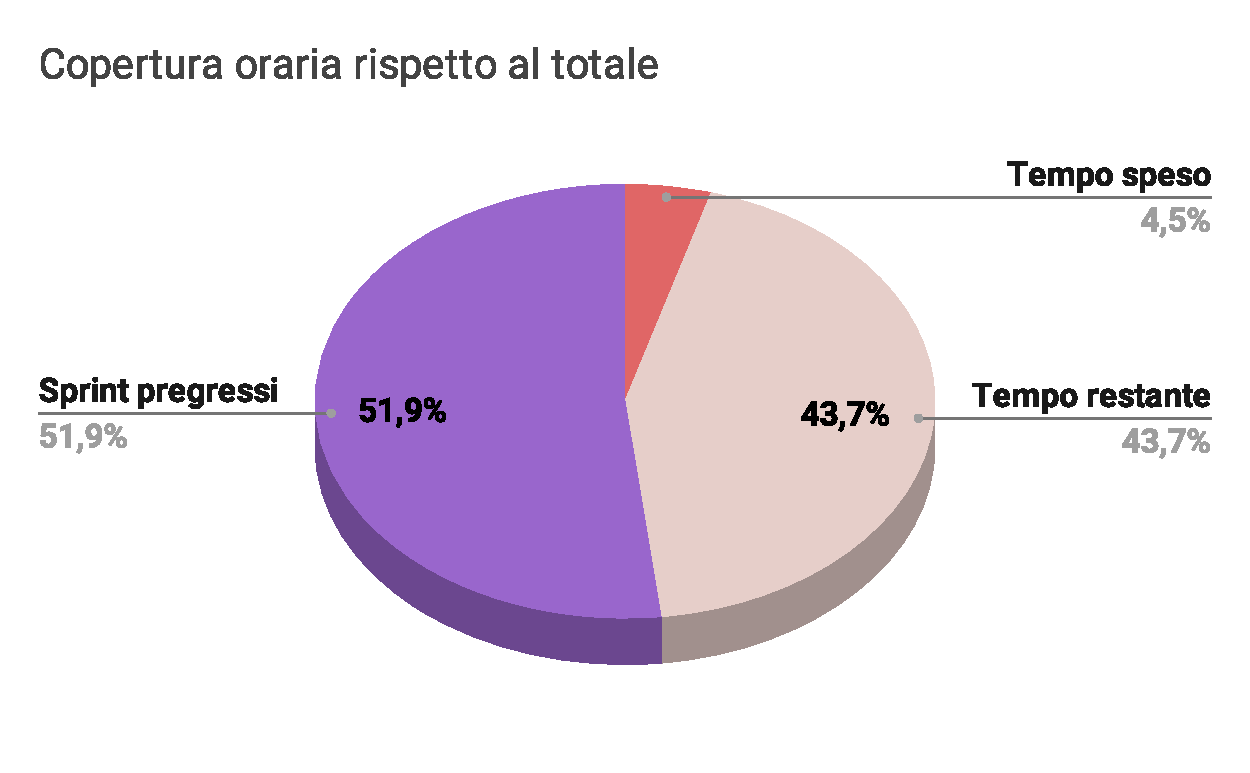
\includegraphics[width=0.90\textwidth]{assets/Consuntivo/Sprint-9/copertura_oraria.pdf}
    \caption{Sprint 10 - Areogramma del tempo speso (in ore) rispetto al totale}
  \end{figure}

  \begin{figure}[H]
    \centering
    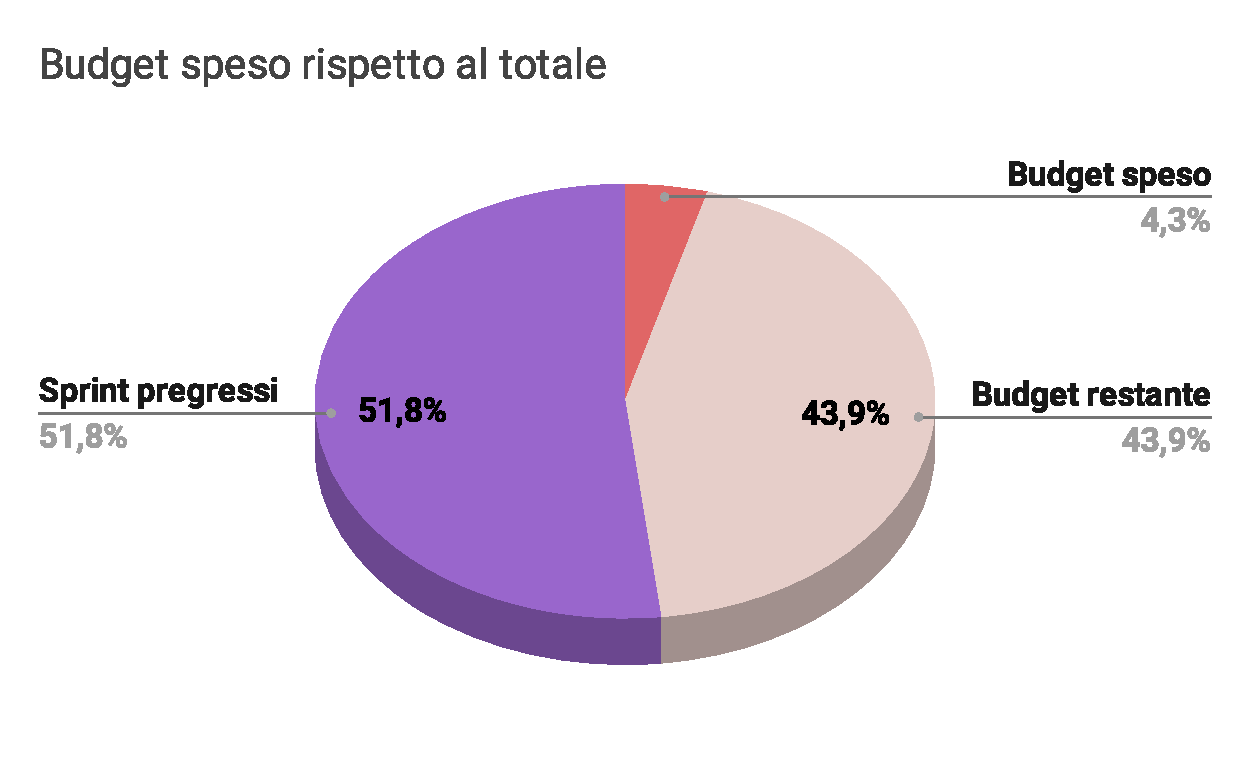
\includegraphics[width=0.90\textwidth]{assets/Consuntivo/Sprint-9/budget_speso.pdf}
    \caption{Sprint 10 - Areogramma del budget speso rispetto al totale}
  \end{figure}

  \begin{minipage}{\textwidth}
    Di seguito sono riportate le ore rimanenti per la coppia risorsa-ruolo:
    \begin{table}[H]
      \begin{tabularx}{\textwidth}{|c|*{6}{>{\centering}X|}c|}
        \hline
        \multicolumn{8}{|c|}{\textbf{Ore rimanenti per la coppia risorsa-ruolo}} \\
        \hline
        \textbf{Membro del team} & \textbf{Re} & \textbf{Am} & \textbf{An} & \textbf{Pt} & \textbf{Pr} & \textbf{Ve} & \textbf{Totale per persona} \\
        \hline
        Cavalli Riccardo & 0 & 0 & 3 & 12 & 10 & 9 & 34 \\
        \hline
        Pianon Raul & 2 & 1 & 1 & 19 & 9 & 6 & 38 \\
        \hline
        Dall’Amico Martina & 2 & 1 & 1 & 14 & 16 & 8 & 42 \\
        \hline
        Cristo Marco & 2 & 4 & 0 & 17 & 10 & 7 & 40 \\
        \hline
        Lewental Sebastiano & 3 & 4 & 1 & 11 & 11 & 11 & 41 \\
        \hline
        Zecchinato Mattia & 5 & 2 & 3 & 9 & 11 & 11 & 41 \\
        \hline
        Stocco Tommaso & 5 & 0 & 3 & 19 & 9 & 8 & 44 \\
        \hline
        \textbf{Totale ore per ruolo} & 19 & 13 & 12 & 101 & 77 & 60 & \textbf{282} \\
        \hline
      \end{tabularx}
      \caption{Sprint 10 - Ore rimanenti per la coppia risorsa-ruolo}
    \end{table}
  \end{minipage}

\subsubsection{Revisione delle attività}

Nell'arco del decimo \glossario{sprint}, il team ha svolto le seguenti attività:
\begin{itemize}
  \item Correzioni alla documentazione post revisione \glossario{RTB};
  \item Stesura verbali interni;
  \item Aggiornamento dei grafici nel \PdQ\;
  \item Miglioramento e formalizzazione delle convenzioni per lo stile di codifica;
  \item Progettazione architetturale \glossario{front-end};
  \item Progettazione logica \glossario{back-end};
  \item Modifica della struttura del front-end;
  \item Valutazione di possibili architetture per il back-end;
  \item Stesura di una relazione sulle architetture individuate;
  \item Progettazione di dettaglio front-end;
  \item Progettazione di dettaglio back-end;
  \item Progettazione del database;
  \item Definizione di nuovi \glossario{dizionario dati};
  \item Selezione degli strumenti di test;
  \item Sperimentazione dei test di unità con pytest e Jest;
  \item Codifica e test di unità front-end;
  \item Configurazione di strumenti di formattazione e linting del codice;
  \item Stesura del documento di \ST;
  \item Stesura del \MU\ (sezioni riguardanti la chat, la gestione dei dizionari e la configurazione delle impostazioni);
  \item Aggiornamento del file \textit{README} e dei requisiti di sistema;
  \item Utilizzo di \glossario{SonarLint} per il calcolo della complessità dei metodi.
\end{itemize}

\subsubsection{Retrospettiva}

\par Di seguito sono riportati i risultati del questionario di valutazione dello \glossario{sprint}:
\begin{itemize}
  \item Organizzazione dello \glossario{sprint}\ - Valutazione: 8;
  \item Conduzione dei meeting interni - Valutazione: 8;
  \item Conduzione dei meeting esterni - Valutazione: 8;
  \item Impegno e partecipazione dei singoli membri - Valutazione: 2.5;
  \item Tutti i membri del gruppo sapevano cosa fare nel loro ruolo;
  \item La numerosità delle riunioni è risultata adeguata per quasi tutti i membri del gruppo;
  \item Le riunioni sono state organizzate sempre con il giusto preavviso;
  \item Il rapporto ore spese/ore produttive è sbilanciato a causa della sessione d'esami;
  \item La produttività è stata comunque ragionevole considerando le criticità della sessione;
\end{itemize}

\vspace{0.5\baselineskip}
\par A seguire le \textbf{analisi a posteriori} del nono \glossario{sprint}:
\begin{itemize}
  \item TODO.
\end{itemize}

\subsubsection{Aggiornamento pianificazione e preventivo}
\par Il team ha definito un piano d'azione per migliorare l'organizzazione e la produttività del prossimo \glossario{sprint}:
\begin{itemize}
  \item TODO.
\end{itemize}

\paragraph*{Pianificazione futura:}
\par TODO.

\paragraph*{Preventivo "a finire" (\sezione{sec:stima_temporale}):}
\par TODO.

\paragraph*{Gestione dei rischi (\sezione{sec:analisi_rischi}):}
\par Durante il nono \glossario{sprint}, i seguenti rischi sono stati gestiti con successo:
\begin{itemize}
  \item \textbf{RT3 - Malfunzionamenti software}: TODO.
\end{itemize}